\documentclass[10pt,a4paper]{article}
%standard symbols
\usepackage{amssymb, amsmath, esint, mathrsfs, tipa}
%charts and tables
\usepackage{array, enumitem}
%graphics
\usepackage{graphicx}
%packages for float
\usepackage{wrapfig, placeins, float}
%specialized tools
\usepackage[americanvoltages,RPvoltages]{circuitikz}
%geometry
\usepackage[left=1.0cm, right=1.0cm, top=2.5cm]{geometry}
%links
\usepackage{hyperref}

\setlength{\textfloatsep}{5pt plus 2pt minus 2pt}
\setlength{\floatsep}{5pt plus 2pt minus 2pt}

\begin{document}

%\tableofcontents

\section{Introduction}

These are a collection of personal notes on the ODMB, an circuit board used by the CMS CSC detectors.

\section{ODMB Firmware}

\subsection{Overall Structure}

The current ODMB is largely split into two pieces The first is ODMB VME (MBV), which executes slow control such as sending commands to DCFEB or LVMB and changing ODMB settings. The second is ODMB CTRL (MBC), which executes fast control needed during data taking.

\subsection{DCFEB JTAG and INITJAG}

The DCFEB JTAG device (cfebjtag.vhd) is the first device in the ODMB VME interface. This module is used to communicate with (x)(D)CFEBs via JTAG protocol (via the PPIB skew clear cables). The signals connecting to this interface are listed in table \ref{tab:cfebjtaginterface}.

\begin{table}[H]
\begin{tabular}{|l|l|} \hline
Port& Description\\ \hline
FASTCLK& 40MHz clock from top level\\ \hline
SLOWCLK& 2.5MHz clock from top level. Called clk\_s1 in odmb\_vme.vhd and top level and said \\
       &to be 10 MHz/0.625 MHz in incorrect comments\\ \hline
RST& Reset signal.\\ \hline
DEVICE& Signal to accept/ignore incoming commands/strobes. Should be connected to DEVICE(1) \\
      & output from COMMAND\_MODULE, which decodes VME commands- will be 1 for \\
			& VME commands 1XXX.\\ \hline 
STROBE& Signal that initiates command execution; generated by COMMAND\_MODULE \\
      & from VME strobe signals\\ \hline
COMMAND& Important bits of VME command (append "00" to end for full command)\\ \hline
WRITER& Unused, connected to WRITER from COMMAND\_MODULE\\ \hline
INDATA& input from directly from VME\_DATA line (through IOBUF)\\ \hline
OUTDATA& output directly to VME\_DATA line (through IOBUF)\\ \hline
DTACK& acknowledge receipt of VME commands, OR'd with DTACKs from other devices \\
     & and sent back to VME\\ \hline
INITJTAGS& signal that resets module and sends signals to reset CFEB JTAG \\
         & state machine, generated when DONE received from (x)(D)CFEBs\\ \hline
TCK& JTAG output to (x)(D)CFEB, one per (x)(D)CFEB\\ \hline
TDI& JTAG output to (x)(D)CFEB, common to all (x)(D)CFEBs\\ \hline
TMS& JTAG output to (x)(D)CFEB, common to all (x)(D)CFEBs\\ \hline
FEBTDO& JTAG input from (x)(D)CFEB, one per (x)(D)CFEBs\\ \hline
LED& DEBUG output, currently clock when shifting header\\ \hline
DIAGOUT& DEBUG output\\ \hline
CSP\_LVMB\_LA\_CTRL& Unused\\ \hline
\end{tabular}
\caption{Signals in CFEBJTAG device}
\label{tab:cfebjtaginterface}
\end{table}

When a STROBE signal is received and there is an appropriate VME command, a LOAD signal is generated, which then generates a BUSY signal. The BUSY signal then causes the global TCK clock to run. It has been observed that sometimes, a `ghost strobe' signal is received, which causes TCK to run with TMS/TDI set to a constant 0. This may result in strange commands being sent to the (x)(D)CFEBs. The appearance of these ghost strobes seem to change with unrelated changes to firmware, indicating a race condition or something similar. 

The TMS signals are generated by loops of sequentially connected D flops. By using FDC(E) and FDP(E) flops, certain sequences of 1's and 0's are achieved in order to control the JTAG state machine. The FD flops from the Latches\_Flipflops package are found not to work on the KCU105 evaluation board and were replaced with the equivalent UNISIM components. Furthermore, the CB4CE and SR16LCE functions from the Latches\_Flipflops package did not defaultly work on the KCU105 evaluation board, and their implementation was slightly tweaked to nest conditions rather than AND'ing them. It is unclear why this changes behavior.

The INITJTAG signal is generated after receiving DONE from the (x)(D)CFEBs. The signal pon\_rst\_reg is initialized to a particular value from PLL\_LOCK when ODMB is reset and after a few clock cycles, pon\_reset becomes '1', which sets done\_current\_state to DONE\_LOW. When the DONE for an (x)(D)CFEB becomes '1', the done\_current\_state is set to DONE\_COUNTING, which generates dcfeb\_done\_pulse. All the dcfeb\_done\_pulse's are OR'd together and converted to a pulse to generate INITJTAG. Perhaps this logic could be moved from the top level to inside of cfebjtag.vhd.

\subsection{Command Module}

The command module (command.vhd) is a helper device in the ODMB VME interface responsible for decoding the signals received from the VME backplane. The signals connecting to this interface are listed in table \ref{tab:commandinterface}.

\begin{table}[H]
\begin{tabular}{|l|l|} \hline
Port& Description\\ \hline
FASTCLK& 40MHz clock from top level\\ \hline
SLOWCLK& 2.5MHz clock from top level\\ \hline
GA& VME geographical address from VME\_GA and VME\_GAP (GA(5) should be VME\_GAP)\\ \hline
ADR& VME address from VME\_ADDR\\ \hline
AM& VME address modifier from VME\_AM\\ \hline
AS& VME address strobe from VME\_AS\_B\\ \hline
DS0& Lower bit of VME data strobe from VME\_DS\_B(0)\\ \hline
DS1& Upper bit of VME data strobe from VME\_DS\_B(1)\\ \hline
LWORD& VME load word from VME\_LWORD\_B\\ \hline
WRITER& VME write signal from VME\_WRITE\_B\\ \hline
IACK& VME interrupt acknowledge from VME\_IACK\_B\\ \hline
BERR& VME error signal from VME\_BERR\_B\\ \hline
SYSFAIL& VME SYSFAIL signal from VME\_SYSFAIL\_B ``1'' indicates OK\\ \hline
TOVME\_B& signal controlling VME\_DATA IOBUF at top level and output as VME\_TOVME\\ \hline
DOE\_B& output as VME\_DOE\_B\\ \hline
DEVICE& each of 10 bits indicates to ODMB VME device if it is selected\\ \hline
STROBE& signal sent to ODMB VME devices to indicate command ready\\ \hline
COMMAND& decoded VME command sent to each ODMB VME device\\ \hline
ADRS& used to multiplex VME\_DATA\_OUT from the various devices\\ \hline
DIAGOUT& for debugging\\ \hline
LED& for debugging\\ \hline
\end{tabular}
\caption{Signals in command module device}
\label{tab:commandinterface}
\end{table}

For more on VME protocol, see \href{http://www.interfacebus.com/Design_Connector_VME.html}{VME Reference}. This device loads AM into AMS when AS is '1'. When DS are both low, AMS is appropriate, and other signals are okay, a strobe is generated.

\subsection{VME Simulation}

The VME simulation is described by the state machine in figure \ref{fig:vmestatemachine}. Although the time-out functionality works in simulation, it works inconsistently on the KCU105 evaluation board. 

\begin{figure}[H]
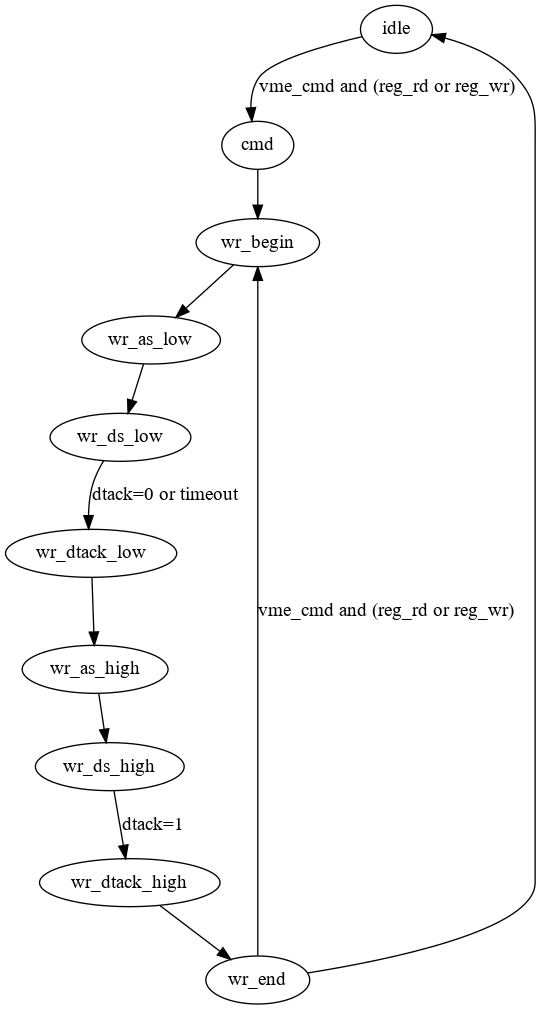
\includegraphics[width= 0.4 \textwidth]{figures/vmestates.png}
\caption{Simulated VME state machine}
\label{fig:vmestatemachine}
\end{figure}

%\bibliography{writeup}
%\bibliographystyle{plain}

\end{document}
